\chapter{Projeto e Implementação}\label{chap:projeto-implementacao}
Este capítulo aborda, com mais detalhes, a parte de projeto e implementação do sistema, com base nos requisitos já levantados, passando pelas tecnologias envolvidas e pela arquitetura do sistema. Além disso, passa pelas etapas que ocorreram, com base no processo levantado no capítulo \ref{chap:metodologia-trabalho}.

\section{Elaboração e Estrutura do Sistema}
Está seção discute os casos de uso do sistema, como eles foram levantados e sua correlação com a arquitetura do sistema.

\subsection{Casos de Uso}
Para levantar os casos de uso, foram realizadas diversas entrevistas com os \textit{stakeholders}.

Primeiramente, um entrevista inicial ocorreu no dia 12/03, com os coordenadores da disciplinas de projeto de formatura: Prof. Dr. João Batista e Prof. Dr. Paulo Cugnasca. Nessa reunião, também teve a participação do Prof. Dr. Fabio Levy Siqueira. Esta entrevista teve dois focos: determinar o processo geral das disciplinas de formatura e encontrar os demais envolvidos que podem ser entrevistados.

Após a primeira entrevista, ocorreram outras conversas entre os demais envolvidos do processo. Foram elas:

\begin{itemize}
    \item Nilton: Responsável técnico dos eventos de banca teórica e feira prática. Evidenciou as necessidades técnicas que possui nos dois dias de evento e deu sugestões de como o sistema pode ajudar em seu trabalho.
    \item Fabio Levy: Assumiu três papéis, por motivos de dificuldade de agenda: Responsável pela infraestrutura de hospedagem, professor orientador e avaliador técnico. Mostrou com mais detalhes o processo como um todo, mas da visão de docente, as participações durante a orientação e a entrega do trabalho de formatura. Além disso, determinou algumas restrições de construção e da infraestrutura do projeto.
\end{itemize}

Após cada entrevista, o processo \textit{AS IS} foi revisto e refinado, obtendo como resultado os diagramas do apêndice \ref{chap:bpmn-appendix}. Com base nesses diagramas, foram construídos os casos de uso do sistema, detalhados no apêndice \ref{chap:use-case-appendix}). 

\subsubsection{Atores dos Casos de Uso}
Para o sistema, temos os seguintes atores:

\begin{itemize}
    \item Alunos: responsáveis por realizar as entregas necessárias das disciplinas.
    \item Professores: realiza a orientação dos alunos e a avaliação das bancas teóricas.
    \item Convidados: realiza a co-orientação dos alunos (se necessário) e a avaliação das bancas práticas.
    \item Técnicos: cuida da gestão dos recursos necessários para os eventos teóricos e práticos.
    \item Coordenadores: gerenciam tudo das disciplinas de projeto de formatura, as entregas, atividades, eventos e centralização das avaliações.
    \item Público: Acessa os recursos públicos, como as monografias finais.
\end{itemize}

\subsubsection{Casos de Uso Implementados}
Os casos de uso implementados foram divididos em duas iterações: uma responsável por gerenciar as atividades ao longo das disciplinas e outra para cuidar dos eventos de avaliação.

\begin{figure}[H]
    \centering
    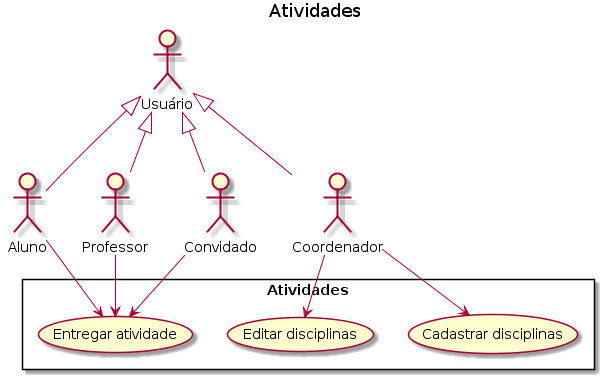
\includegraphics[scale=0.6]{atv.png}
    \caption{Diagrama de Casos de Uso para Atividades}
    \label{fig:use-case-atv}
\end{figure}

\begin{figure}[H]
    \centering
    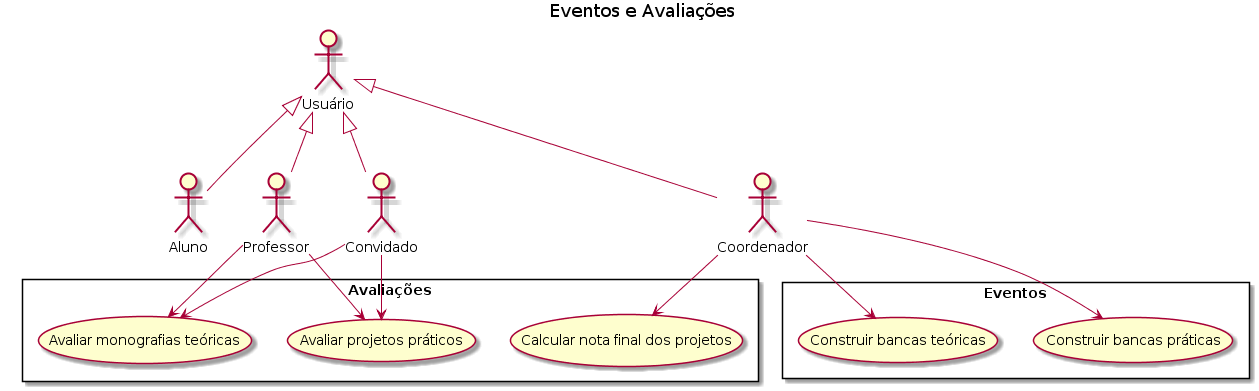
\includegraphics[scale=0.3]{ev-ava.png}
    \caption{Diagrama de Casos de Uso para Eventos e Avaliações}
    \label{fig:use-case-ev-ava}
\end{figure}

\begin{figure}[H]
    \centering
    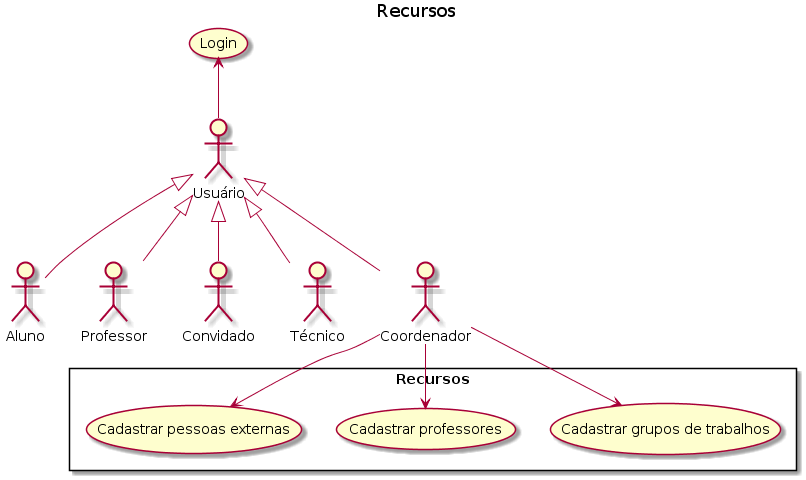
\includegraphics[scale=0.5]{recursos.png}
    \caption{Diagrama de Casos de Uso para Gerenciamento dos Recursos}
    \label{fig:use-case-recursos}
\end{figure}

Com os diagramas de caso de uso, agora há a descrição dos casos de uso implementados, divididos por iteração:

\begin{itemize}
    \item Primeira Iteração - Julho/Setembro
    \begin{itemize}
        \item Login: Alunos, Orientadores, Co-orientadores e Coordenadores acessam sistema de maneira tradicional ou via Senha Única USP (para pertencentes à USP).
        \item Cadastrar disciplinas: Coordenadores cadastram a disciplina, os alunos participantes e as atividades.
        \item Editar disciplinas: Coordenadores editam disciplinas, cadastrando atividades, editando alunos etc.
        \item Cadastrar grupos de trabalhos: Coordenadores cadastram os grupos com os temas e os orientadores, com a confirmação da participação do orientador no grupo.
        \item Cadastrar professores: Coordenadores cadastram professores do departamento que podem orientar/co-orientar.
        \item Cadastrar pessoas externas: Coordenadores cadastram convidados do sistema que podem avaliar projetos nas bancas práticas e/ou co-orientar.
        \item Entregar atividade: Alunos submetem no Google Drive arquivos da atividade para a leitura do orientador, co-orientador e coordenadores.
    \end{itemize}
\end{itemize}

\begin{itemize}
    \item Segunda Iteração - Outubro/Novembro
    \begin{itemize}
        \item Listar entregas: Técnicos recebem os arquivos de impressão, com normalização do título, separados por grupo.
        \item Listar necessidades adicionais: Técnicos recebem necessidades adicionais revisadas pelos orientadores, separadas por grupo.
        \item Construir bancas práticas: Coordenadores selecionam os participantes da banca prática, já cadastrados no sistema, e os notifica com comentários sobre o evento.
        \item Construir bancas teóricas: Coordenadores escolhem participantes da banca teórica do grupo, selecionam o presidente da banca, realizam o agendamento do horário, validando inconsistências (participante já possui horário ocupado) e notificam os participantes por e-mail.
        \item Avaliar projetos práticos: Participantes da banca prática avaliam os projetos que estão envolvidos, limitando avaliações até o final do dia.
        \item Avaliar monografias teóricas: Participantes da banca teórica avaliam as monografias que estão envolvidas, gerando comentários e definindo o status do trabalho (aprovado, aprovado com correções, recuperação e reprovado), limitando avaliações até o final do dia.
        \item Calcular nota final dos projetos: Coordenadores determinam a fórmula para calcular as notas finais, com base nas entregas parciais durante as duas disciplinas e o sistema calcula as notas finais de todos os grupos participantes.
    \end{itemize}
\end{itemize}

Cada iteração teve sua reunião de validação dos casos de uso: a primeira no dia 4/4 e a segunda no dia 30/10.

\subsubsection{Casos de Uso não implementados}
Há também os casos de uso não implementados do sistema, levantados como perspectivas de continuidade do sistema. São eles:

\begin{itemize}
    \item Importar projetos aprovados: Sistema importa monografias revisadas, banners, press-releases, posters e links do site para a base de dados históricos de TCC.
    \item Cadastrar projetos avulsos: Coordenadores cadastram monografias revisadas, banners, press-releases, posters e links do site de trabalhos anteriores para a base de dados históricos de TCC.
    \item Propor tema de trabalho: Alunos e Orientadores propõem temas em busca de orientadores ou alunos dispostos a realizarem.
    \item Buscar projetos anteriores: Usuários externos ao sistema procuram monografias anteriores, de acordo com o nome, ano, turma (semestral ou quadrimestral) e palavras-chave.
    \item Buscar temas propostos: Alunos e orientadores procuram temas propostos por outros alunos e orientadores, de acordo com o nome, palavras-chave e grupos de pesquisa do departamento, podendo se inscrever nas vagas para esses temas (se houverem).
\end{itemize}

\begin{figure}[H]
    \centering
    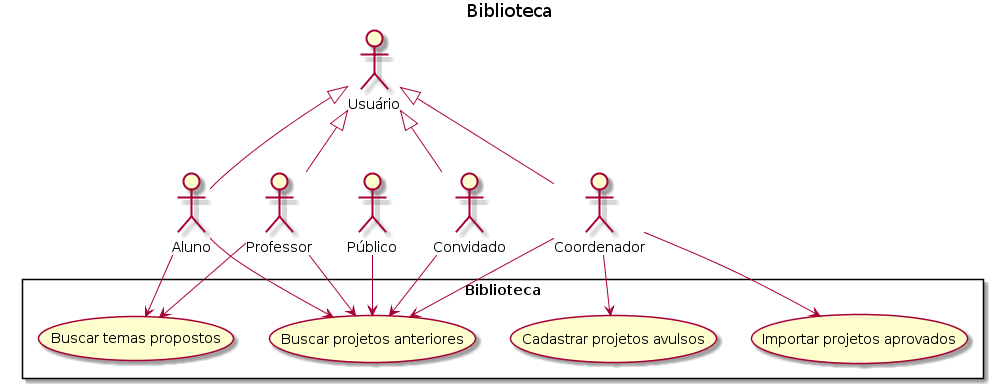
\includegraphics[scale=0.4]{bib.png}
    \caption{Diagrama de Casos de Uso para Base de Dados (Biblioteca Virtual)}
    \label{fig:use-case-bib}
\end{figure}

\begin{figure}[H]
    \centering
    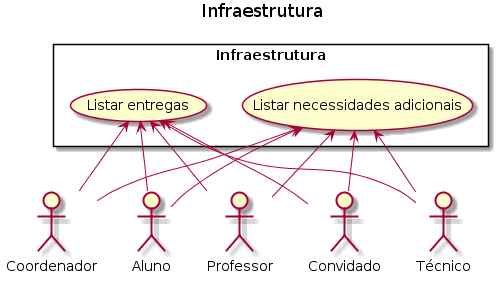
\includegraphics[scale=0.6]{infra.png}
    \caption{Diagrama de Casos de Uso para Infraestrutura}
    \label{fig:use-case-infra}
\end{figure}

\section{Arquitetura e Tecnologias Utilizadas}

\begin{figure}[H]
    \centering
    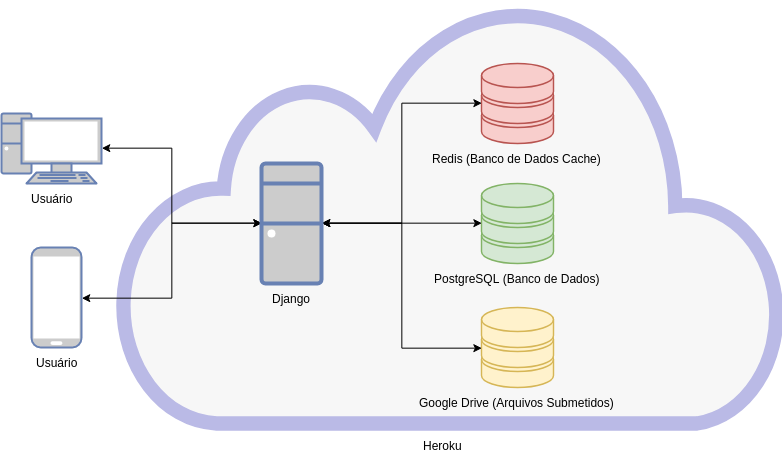
\includegraphics[scale=0.4]{arquitetura.png}
    \caption{Arquitetura Básica do Sistema}
    \label{fig:arch}
\end{figure}

É comum, em desenvolvimento de sistemas, usar soluções prontas como forma de simplificar o desenvolvimento de soluções. Essas soluções são conhecidas como arcabouços (ou \textit{frameworks}), definidos por \citeauthor{iansommerville2011} como: "uma estrutura genérica estendida para se criar uma aplicação ou subsistema mais específico". Para este projeto, foi usado um \textit{framework}, em linguagem Python, chamado \textbf{Django}. Sua escolha foi pautada na Manutenibilidade, levantada no capítulo \ref{chap:especificacao-requisitos-sistema}, dado que alunos farão a manutenção do projeto e que Python, além de ser mais alto nível, é ensinada no primeiro ano dos cursos de Engenharia da Poli.

O Django é estruturado em aplicações (apps), onde cada aplicação corresponde a uma parte do sistema, geralmente independente e reciclável (ou seja, pode ser usada em aplicações Django diferentes). Cada aplicação segue o padrão \textit{Model-View-Controller}.

O padrão \textit{Model-View-Controller} - MVC é um padrão arquitetural para organizar os componentes da aplicação. Ele é dividido em três grandes grupos\cite{thedjangobook2018}:

\begin{itemize}
    \item Modelo (\textit{Model}): Fonte de informação, contendo os dados da aplicação, é onde geralmente fica a lógica de negócio.
    \item Visualização (\textit{View}): Camada de apresentação dos dados da aplicação. No caso do Django, ele é chamado de \textit{Template}.
    \item Controlador (\textit{Controller}): Camada de controle que interliga o modelo com a apresentação dos dados. No caso do Django, ele é conhecido como \textit{View}.
\end{itemize}

A vantagem do padrão está no fluxo de dados que existe entre os grupos, além de evitar códigos com funcionalidades diferentes em lugares errados, como, por exemplo, lógica de negócio na camada de apresentação.

Já para a hospedagem, foi usado como apoio o Heroku, um serviço de plataforma (\textit{Platform as a Service} - \textbf{PaaS}) de computação em nuvem conhecida no mercado, com a possibilidade de subir aplicações nas linguagens Ruby, Node.js, Java, Python, Clojure, Scala, Go e PHP. O Heroku foi escolhido pela facilidade em subir uma aplicação gratuitamente, o que possibilita testar e validar ideias básicas. A estrutura básica do Heroku funciona com o uso de \textit{dynos}, que são pequenas máquinas tanto para hospedar sua aplicação principal quanto outras auxiliares para serviços externos e/ou paralelos. Resumidamente, ele possui um plano básico gratuito que possibilita testar aplicações de maneira fácil e sem dificuldades de expansão e, se desejar, há máquinas de performance superior, cobradas com base no conceito de \textit{dynos}-hora.

Mesmo com um dos requisitos sendo a hospedagem em um serviço de nuvem da USP, para realizar as outras etapas dos demais ambientes de desenvolvimento citados no capítulo \ref{chap:metodologia-trabalho}, foram usados três ambientes (desenvolvimento, homologação e produção) do Heroku, com os seguintes domínios:

\begin{itemize}
    \item Desenvolvimento: \href{https://tccapp-next-release.herokuapp.com}{https://tccapp-next-release.herokuapp.com}
    \item Homologação: \href{https://tccapp-staging.herokuapp.com}{https://tccapp-staging.herokuapp.com}
    \item Produção: \href{https://tccapp-production.herokuapp.com}{https://tccapp-production.herokuapp.com}
\end{itemize}

O Django foi usado na versão mais recente estável (2.1), que corrigiu algumas novidades da versão 2.0. É esta versão que foi usada pelo projeto em questão, dado que é estável e possui suporte de apoio da equipe até Dezembro de 2020\cite{djangodownload}. Ele usa, como padrão, o SQLite, o que atendeu bem durante o desenvolvimento. Já o Heroku tem como banco de dados padrão o PostgreSQL, o que exigiu o chaveamento entre os bancos no ambiente local de desenvolvimento e os ambientes de validação hospedados no serviço. Por isso, o projeto possui configurado dois pacotes de gerenciamento de banco de dados, um para SQLite (nativo do Django), outro para PostgreSQL (o Psycopg\cite{lucassouto2017}).

Em relação aos acessos do sistema, o Django possui uma limitação (caso use o serviço nativo de login): apenas um \textit{model} pode realizar o acesso. Como são múltiplos atores, para contornar a limitação, cada pessoa terá um único usuário, com vários perfis diferentes de acesso, cada qual com suas permissões e ações. São quatro perfis implementados: estudante, docente, convidado e coordenador. Cada usuário pode ter um ou mais perfis de acesso simultâneos (é o caso, por exemplo, dos coordenadores da disciplina, que também são docentes e podem orientar e avaliar projetos).

\subsection{Aplicações Construídas}
O Django possui uma filosofia em sua documentação\cite{djangodocs}: "Uma aplicação é um aplicativo da Web que faz alguma coisa - por exemplo, um sistema de blog, um banco de dados de registros públicos ou um aplicativo de pesquisa simples. Um projeto é uma coleção de configurações e aplicações para um site específico." Seguindo essa filosofia definida, o sistema foi estruturado em aplicações menores \textit{apps}, cada qual com sua responsabilidade:

\begin{itemize}
    \item home: Aplicação responsável por gerenciar as funções básicas a todos os usuários, como por exemplo login/logout, o conteúdo da página de entrada, entre outros.
    \item users: Gerencia os usuários cadastrados do sistema e os seus perfis (aluno, docente, convidado e coordenador)
    \item disciplines: Gerencia as disciplinas de TCC do curso, duas disciplinas por ano (TCC1 e TCC2).
    \item activities: Gerencia as atividades das diversas disciplinas do sistema.
    \item workgroups: Cuida dos grupos de trabalho criados durante as disciplinas. 
    \item deliveries: Cuida das entregas das atividades do curso, cada uma realizada pelos grupos de trabalho e revisadas pelos orientadores/co-orientadores.
    \item rooms: Cuida das salas que serão usadas nos eventos de bancas teóricas e práticas.
    \item events: Gerencia os eventos teóricos e práticos que ocorrem nas disciplinas de TCC2.
    \item allocations: Cuida das alocações de cada grupo, para cada evento teórico ou prático, junto com os convidados e docentes que avaliarão o grupo.
    \item evaluations: Gerencia as avaliações que cada docente ou convidado alocado fará nos eventos.
    \item rules: Determina as disciplinas e os eventos que serão usados para calcular as notas finais.
    \item score: Gerencia as notas finais calculadas para cada situação, por grupo de trabalho.
\end{itemize}

Com as aplicações estabelecidas, os dados foram organizados na arquitetura de banco de dados a seguir:

\begin{figure}[H]
    \centering
    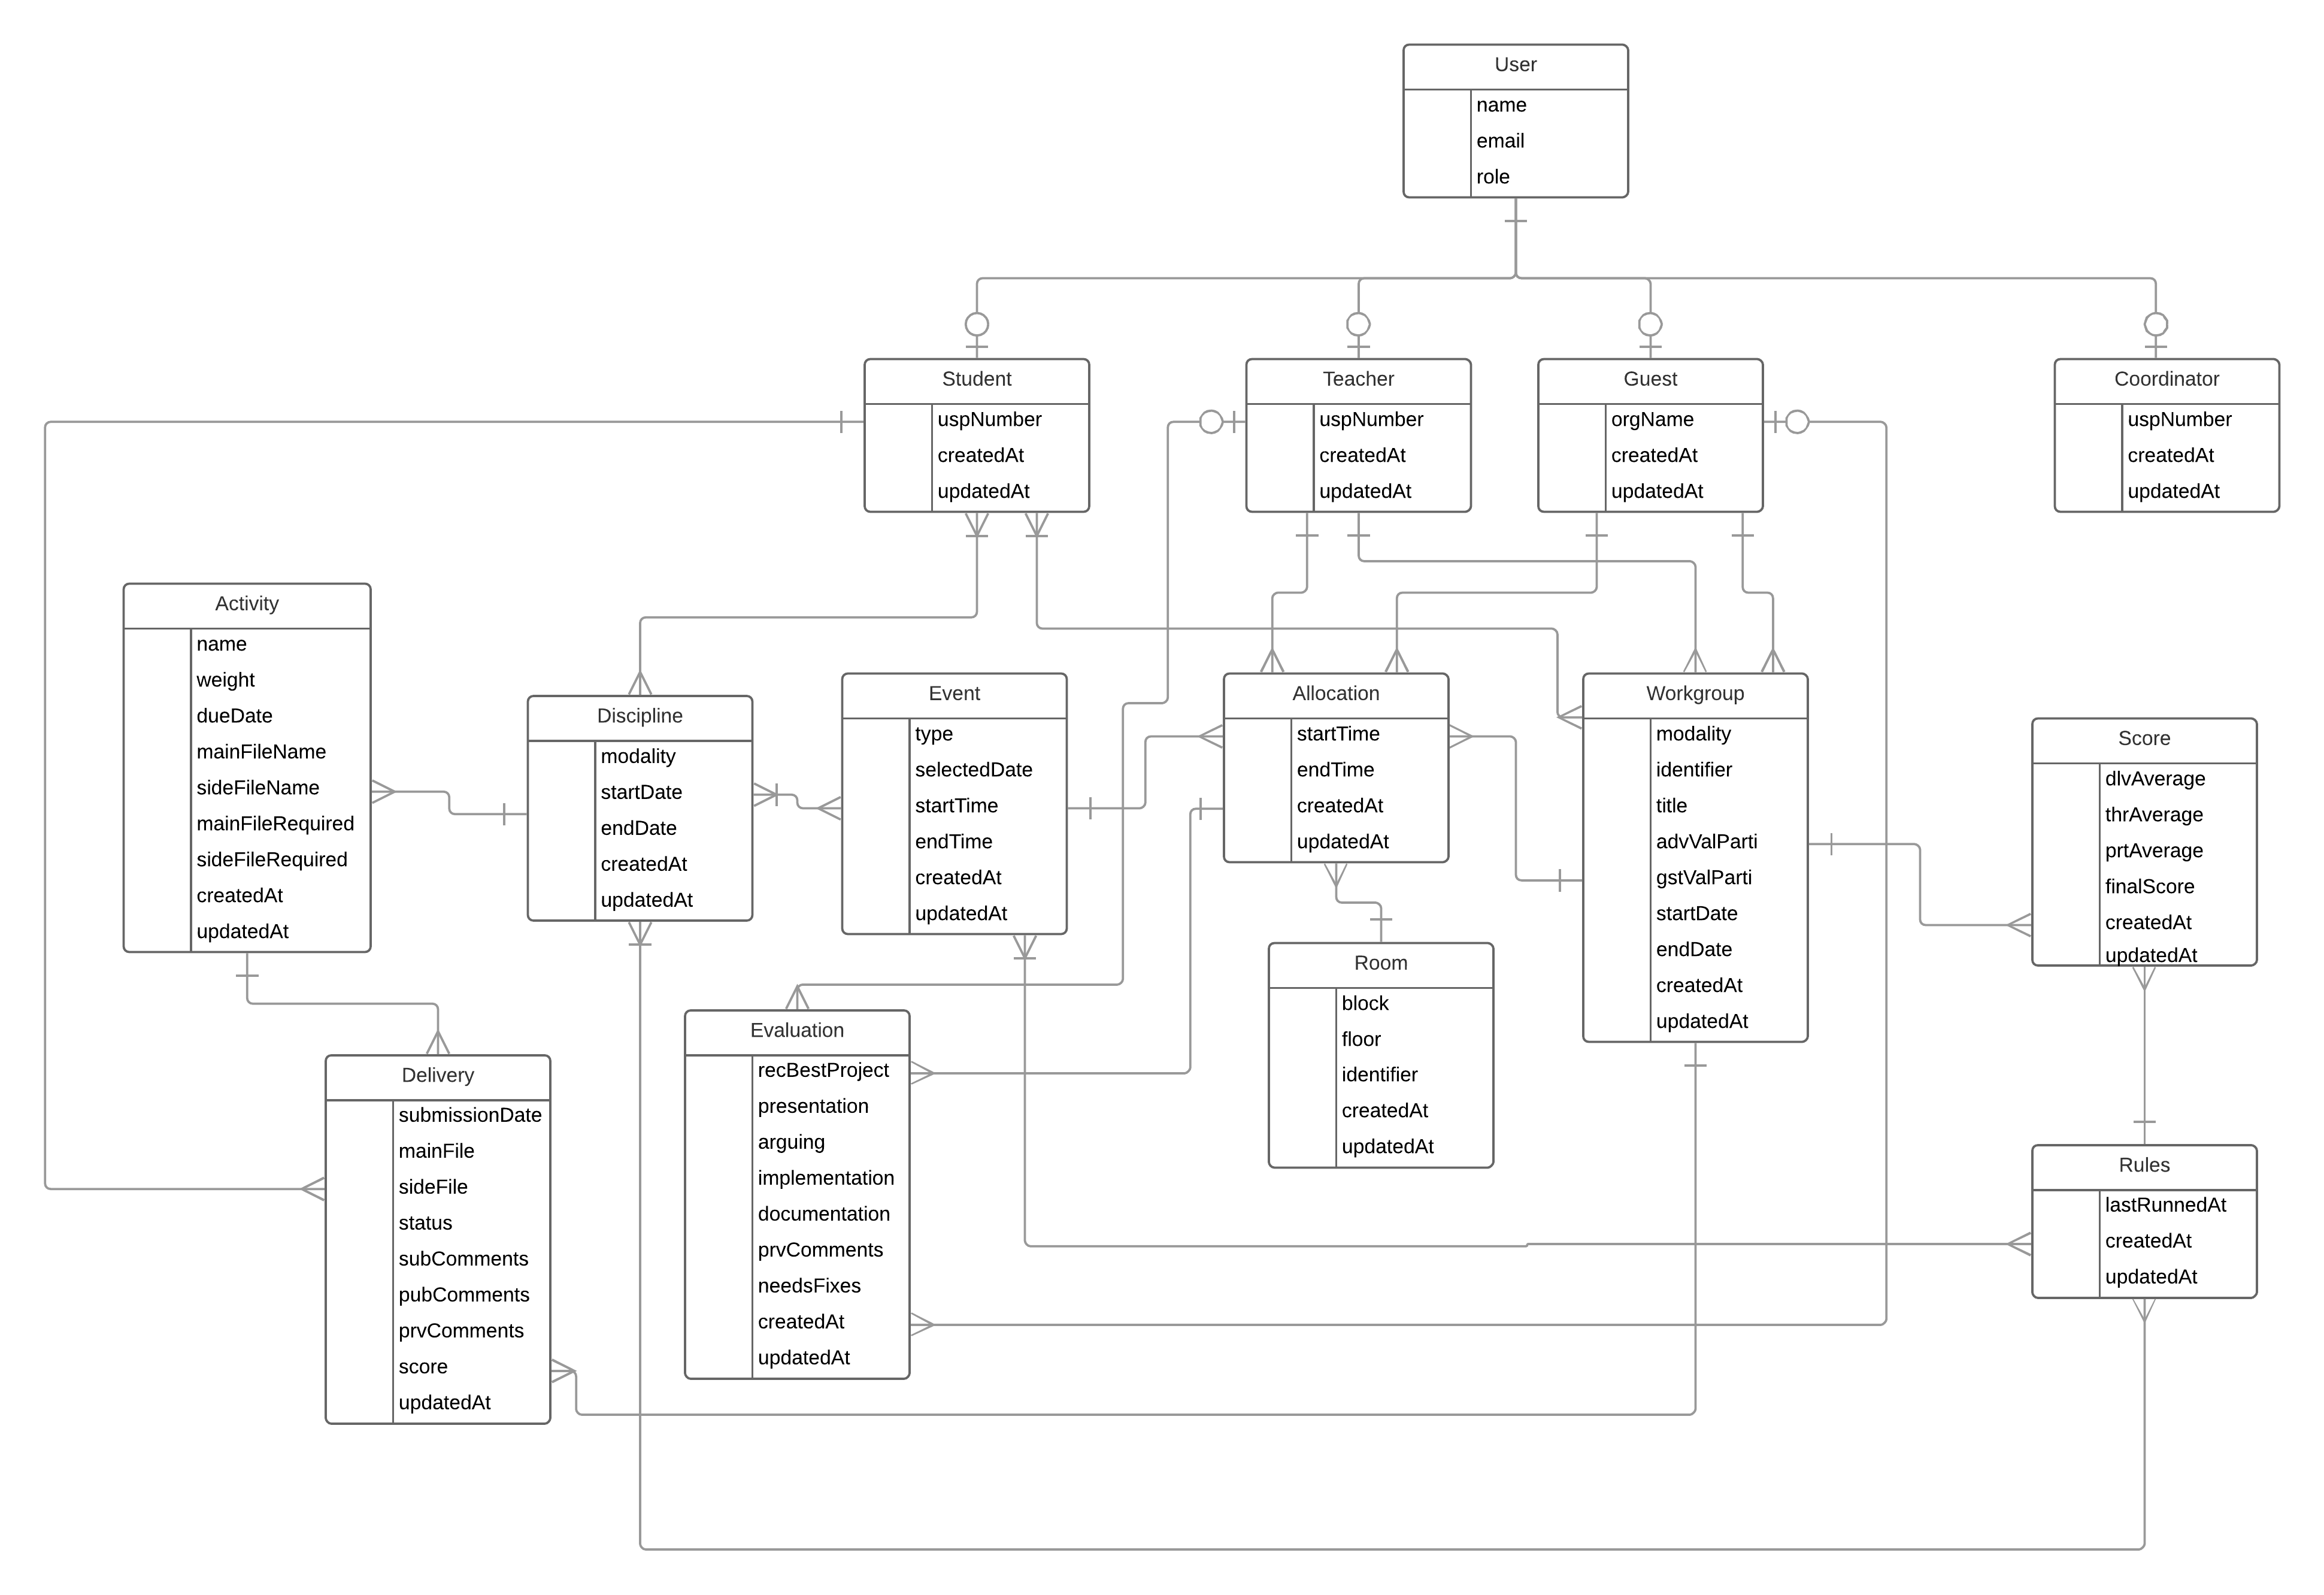
\includegraphics[angle=90, origin=c, scale=0.65]{imagens/erd.png}
    \caption{Diagrama Entidade-Relacionamento em Nível Lógico do Sistema Desenvolvido, usando Notação de Pé de Galinha}
    \label{fig:erd}
\end{figure}

Para a navegação de telas, foram construídos diagramas de navegação simples, exibindo a arquitetura de informação do sistema para cada perfil de usuário:

\begin{figure}[H]
    \centering
    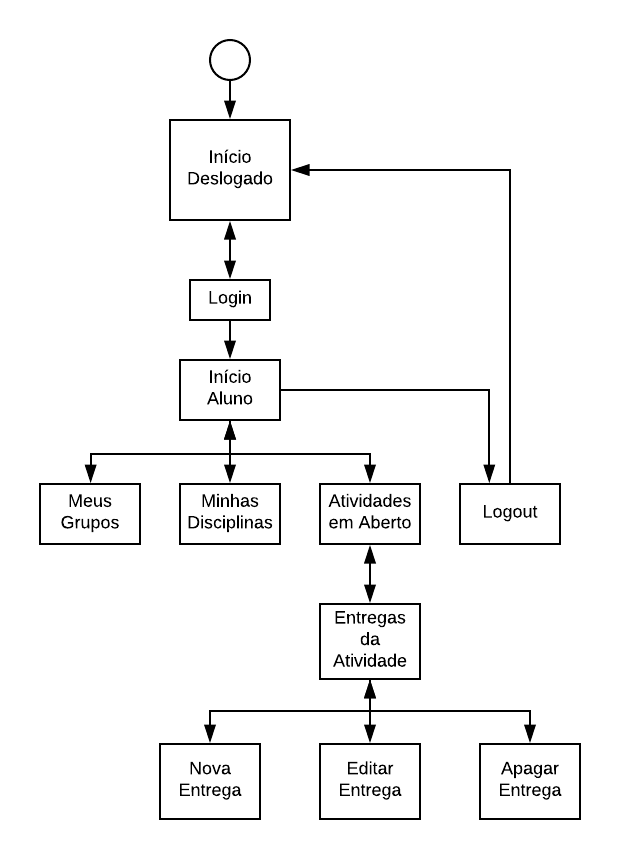
\includegraphics[scale=1]{imagens/telas_aluno.png}
    \caption{Diagrama de Navegação de Telas Simplificado para o perfil de Aluno}
    \label{fig:telas-aluno}
\end{figure}

\begin{figure}[H]
    \centering
    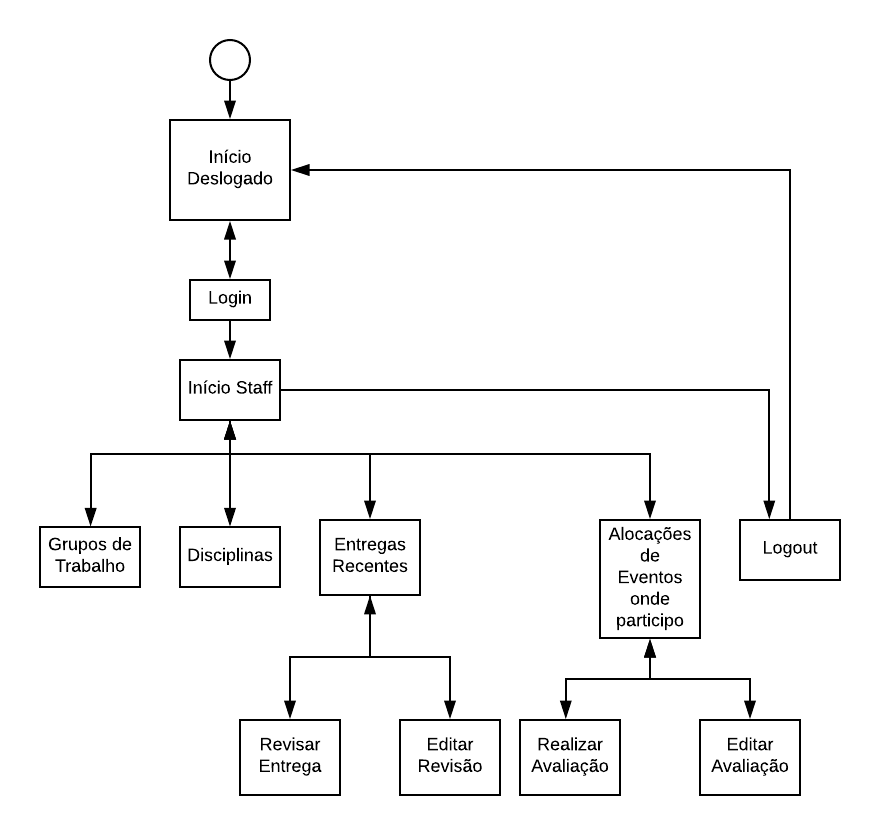
\includegraphics[scale=1]{imagens/telas_staff.png}
    \caption{Diagrama de Navegação de Telas Simplificado para o perfis de Docente e Convidado}
    \label{fig:telas-staff}
\end{figure}

\begin{figure}[H]
    \centering
    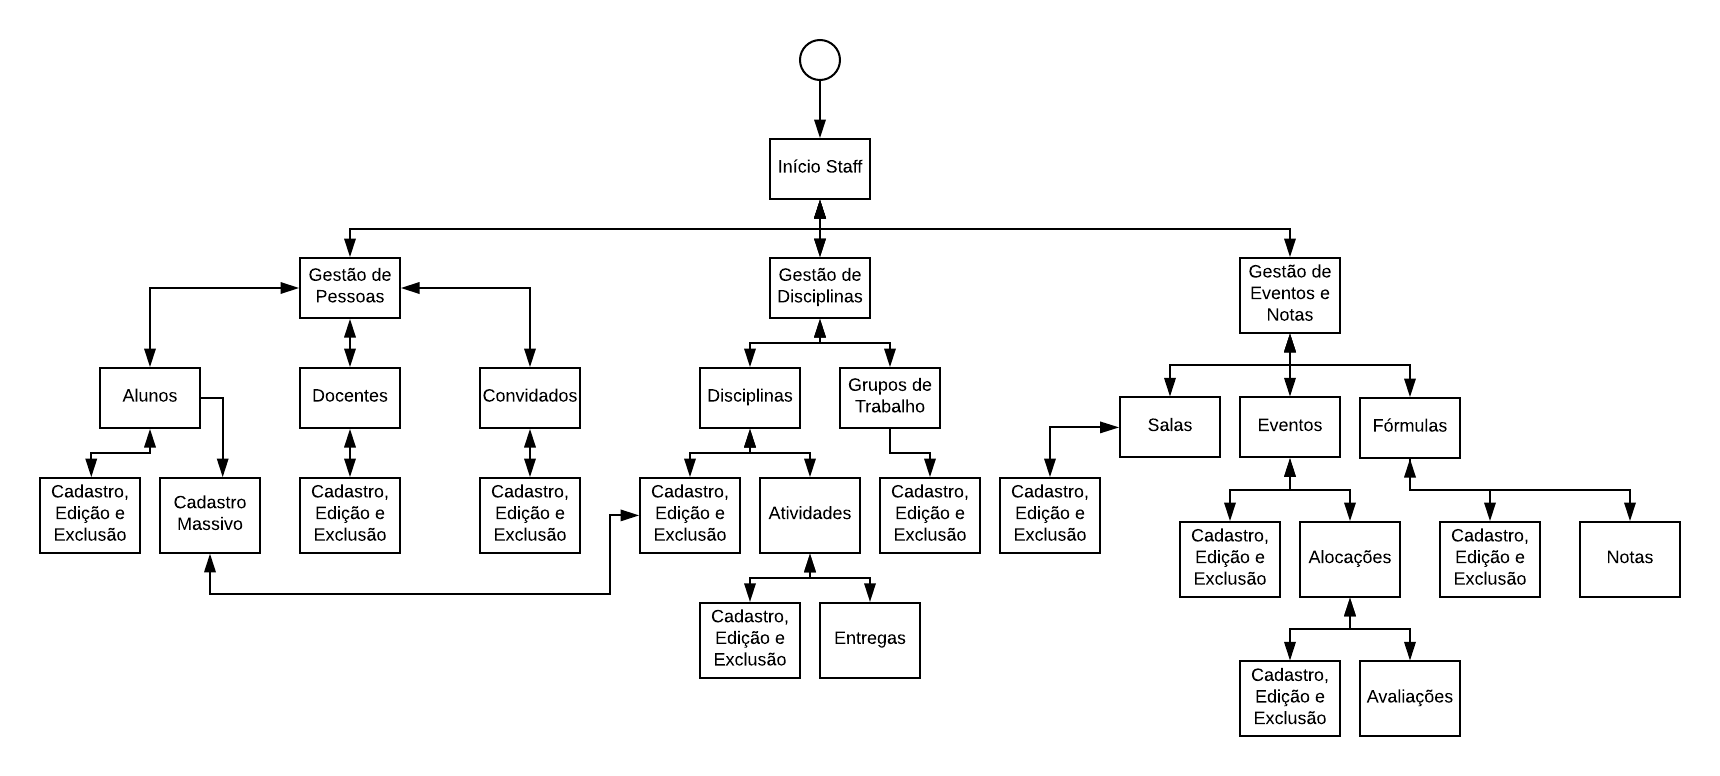
\includegraphics[angle=90, origin=c,scale=0.7]{imagens/telas_coordenador.png}
    \caption{Diagrama de Navegação de Telas Simplificado para o perfil de Coordenador}
    \label{fig:telas-coordenador}
\end{figure}

De forma a evitar excesso de conteúdo no trabalho, todo o código presente está em um repositório público na plataforma de controle de versão GitHub, onde também se encontram detalhes mais técnicos sobre como realizar manutenções no sistema e como rodar na máquina do desenvolvedor: \href{https://github.com/LucasArthur94/tccapp}{https://github.com/LucasArthur94/tccapp}.

Há também, no anexo \ref{chap:user-manual-appendix}, um pequeno manual de instruções de uso do sistema, com algumas capturas de tela para ilustrar o fluxo de navegação para os diversos atores.